\chapter{Base Camp Dashboard}
\label{ch:dashboard}

The Base Camp Dashboard is a robust Python Flask application designed to run on a laptop at the expedition's base camp. It serves as the central hub for monitoring all climbers on the mountain, visualizing their locations, tracking health vitals, and managing emergency communications.

\section{System Requirements and Launching}

The dashboard is packaged as a standalone desktop application using PyInstaller, ensuring it can run without a complex Python environment setup in the field.

\subsection{Launching the Application}
\begin{enumerate}
    \item Locate the executable file (\texttt{SummitGear\_Dashboard.exe} on Windows or \texttt{SummitGear\_Dashboard.app} on macOS).
    \item Double-click to launch the application.
    \item The application will start a local Flask server and open the default web browser to \texttt{http://127.0.0.1:5000}.
\end{enumerate}

\subsection{Hardware Connection}
The dashboard requires a connection to the Base Camp Unit (ESP32) to receive LoRa transmissions from the climbers.

\begin{enumerate}
    \item Connect the Base Camp Unit to the laptop using a high-quality USB data cable.
    \item Ensure the device is powered on.
\end{enumerate}

\section{Connecting to the Base Camp Unit}

Once the dashboard is running and the hardware is connected, you must establish a serial connection.

\begin{enumerate}
    \item In the dashboard interface, locate the \textbf{Connection Settings} panel in the top-right corner.
    \item Click the \textbf{Scan Ports} button to detect available serial ports.
    \item Select the correct port from the dropdown menu (e.g., \texttt{COM3} on Windows or \texttt{/dev/ttyUSB0} on macOS/Linux).
    \item Verify the baud rate is set to \textbf{115200}.
    \item Click \textbf{Connect}. The status indicator should turn green, indicating successful communication.
\end{enumerate}

\begin{tipbox}
If you are unsure which port corresponds to the Base Camp Unit, disconnect the USB cable, click 'Scan Ports', note the list, reconnect the cable, and scan again. The new port that appears is the correct one.
\end{tipbox}

\begin{figure}[H]
    \centering
    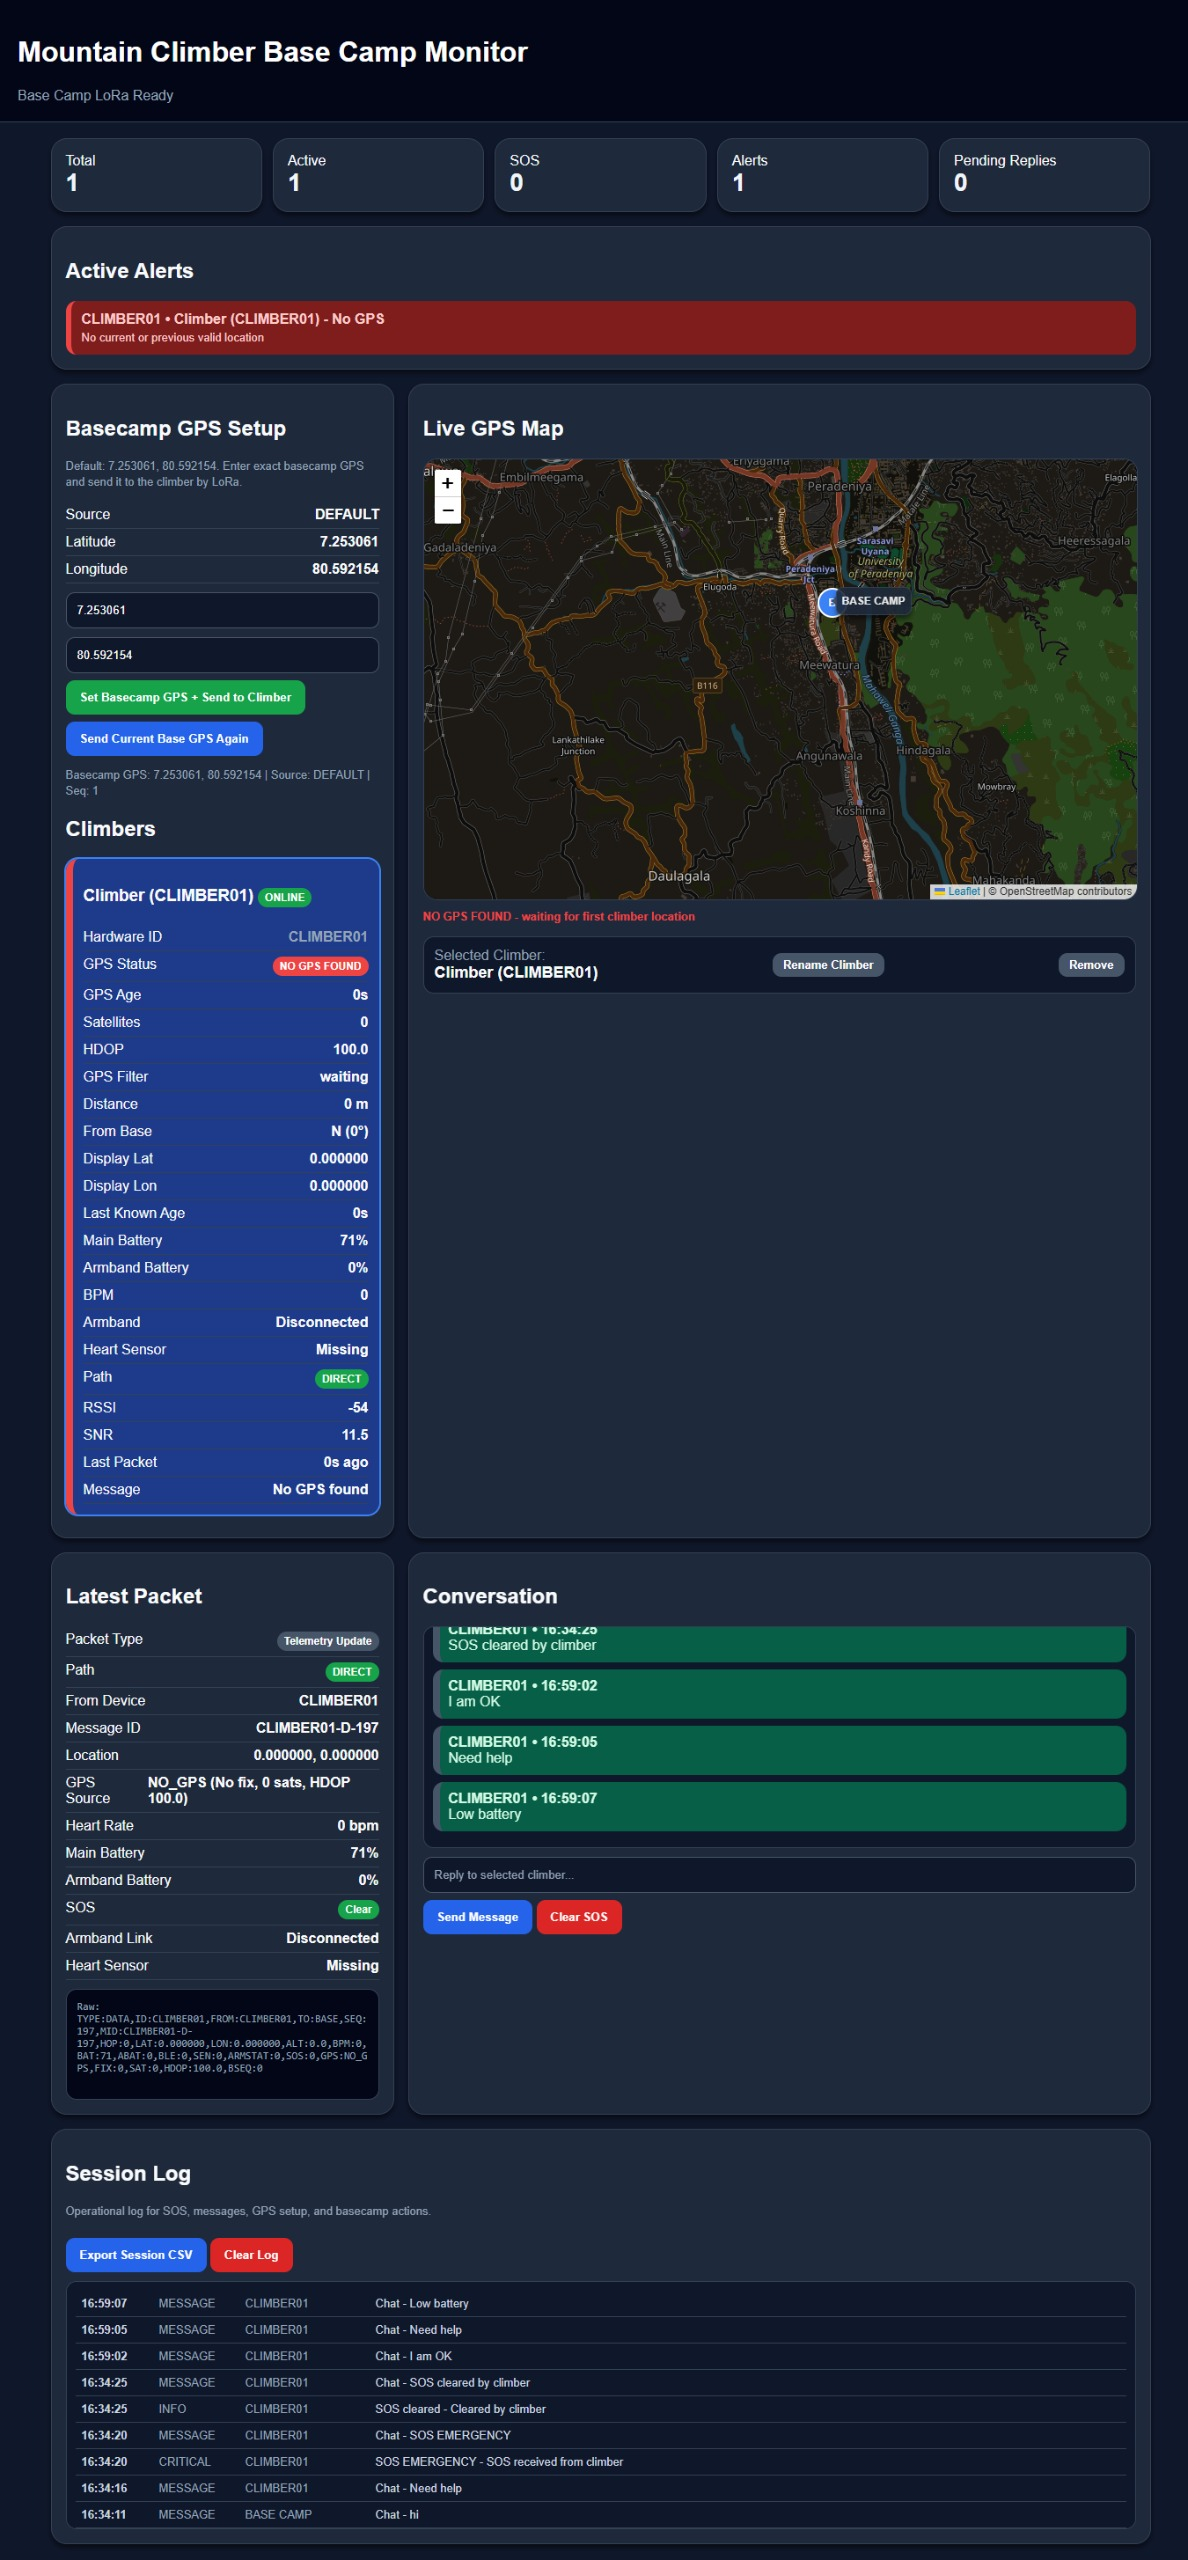
\includegraphics[width=0.9\textwidth]{figures/dashboard-main.png}
    \caption{Base Camp Dashboard Main Interface}
    \label{fig:dashboard-main}
\end{figure}

\section{Monitoring Operations}

\subsection{Real-Time Canvas Map}
The centerpiece of the dashboard is an HTML5 Canvas map that dynamically visualizes the expedition's status based on incoming JSON serial packets.

\begin{itemize}
    \item \textbf{Climber Positions:} Each active climber is represented by an icon on the map.
    \item \textbf{Distances and Bearings:} Hovering over a climber's icon displays their distance and bearing relative to the base camp.
    \item \textbf{Path Tracking:} A trail shows the historical path of each climber during the current session.
\end{itemize}

\subsection{Monitoring Vitals Panel}
To the right of the map, the \textbf{Vitals Panel} provides a tabular view of all connected climbers.

\begin{itemize}
    \item Displays real-time Heart Rate, SpO2, and Temperature.
    \item Values that fall outside predefined safe thresholds (e.g., SpO2 below 85\%) are highlighted in amber or red.
\end{itemize}

\section{Emergency and Communication Management}

\subsection{Handling SOS Alerts}
When a climber triggers an SOS (either manually via a button press or automatically due to critical vitals), the dashboard reacts immediately:

\begin{itemize}
    \item \textbf{Visual Notification:} The screen flashes red, and a modal dialog appears detailing which climber needs assistance and their exact GPS coordinates.
    \item \textbf{Audio Alarm:} A loud audio alert sounds through the laptop speakers to ensure the base camp operator's attention.
    \item \textbf{Action Required:} The operator must click \textbf{Acknowledge} to silence the alarm, which also sends a confirmation message back to the climber's device.
\end{itemize}

\begin{cautionbox}
Always ensure laptop speakers are unmuted and the volume is adequate to hear SOS alarms in a noisy base camp environment.
\end{cautionbox}

\subsection{Messaging Climbers}
Two-way communication is supported via the dashboard's messaging interface.

\begin{enumerate}
    \item Select a specific climber from the dropdown or choose 'Broadcast to All'.
    \item Type your message.
    \item Click \textbf{Send}. The Base Camp Unit will transmit the message over the LoRa network.
\end{enumerate}

\section{Data Management}

\subsection{Exporting Data to CSV}
For post-expedition analysis, auditing, or medical review, the dashboard logs all incoming telemetry data.

\begin{enumerate}
    \item Navigate to the \textbf{Data Management} tab.
    \item Select a date range or a specific climber ID.
    \item Click \textbf{Export to CSV}.
    \item Choose a save location on your laptop. The resulting file will contain timestamps, GPS coordinates, and health vitals for the selected criteria.
\end{enumerate}
